% Options for packages loaded elsewhere
\PassOptionsToPackage{unicode}{hyperref}
\PassOptionsToPackage{hyphens}{url}
\PassOptionsToPackage{dvipsnames,svgnames,x11names}{xcolor}
%
\documentclass[
]{article}

\usepackage{amsmath,amssymb}
\usepackage{iftex}
\ifPDFTeX
  \usepackage[T1]{fontenc}
  \usepackage[utf8]{inputenc}
  \usepackage{textcomp} % provide euro and other symbols
\else % if luatex or xetex
  \usepackage{unicode-math}
  \defaultfontfeatures{Scale=MatchLowercase}
  \defaultfontfeatures[\rmfamily]{Ligatures=TeX,Scale=1}
\fi
\usepackage{lmodern}
\ifPDFTeX\else  
    % xetex/luatex font selection
\fi
% Use upquote if available, for straight quotes in verbatim environments
\IfFileExists{upquote.sty}{\usepackage{upquote}}{}
\IfFileExists{microtype.sty}{% use microtype if available
  \usepackage[]{microtype}
  \UseMicrotypeSet[protrusion]{basicmath} % disable protrusion for tt fonts
}{}
\makeatletter
\@ifundefined{KOMAClassName}{% if non-KOMA class
  \IfFileExists{parskip.sty}{%
    \usepackage{parskip}
  }{% else
    \setlength{\parindent}{0pt}
    \setlength{\parskip}{6pt plus 2pt minus 1pt}}
}{% if KOMA class
  \KOMAoptions{parskip=half}}
\makeatother
\usepackage{xcolor}
\usepackage[margin=0.5in]{geometry}
\setlength{\emergencystretch}{3em} % prevent overfull lines
\setcounter{secnumdepth}{-\maxdimen} % remove section numbering
% Make \paragraph and \subparagraph free-standing
\makeatletter
\ifx\paragraph\undefined\else
  \let\oldparagraph\paragraph
  \renewcommand{\paragraph}{
    \@ifstar
      \xxxParagraphStar
      \xxxParagraphNoStar
  }
  \newcommand{\xxxParagraphStar}[1]{\oldparagraph*{#1}\mbox{}}
  \newcommand{\xxxParagraphNoStar}[1]{\oldparagraph{#1}\mbox{}}
\fi
\ifx\subparagraph\undefined\else
  \let\oldsubparagraph\subparagraph
  \renewcommand{\subparagraph}{
    \@ifstar
      \xxxSubParagraphStar
      \xxxSubParagraphNoStar
  }
  \newcommand{\xxxSubParagraphStar}[1]{\oldsubparagraph*{#1}\mbox{}}
  \newcommand{\xxxSubParagraphNoStar}[1]{\oldsubparagraph{#1}\mbox{}}
\fi
\makeatother

\usepackage{color}
\usepackage{fancyvrb}
\newcommand{\VerbBar}{|}
\newcommand{\VERB}{\Verb[commandchars=\\\{\}]}
\DefineVerbatimEnvironment{Highlighting}{Verbatim}{commandchars=\\\{\}}
% Add ',fontsize=\small' for more characters per line
\newenvironment{Shaded}{}{}
\newcommand{\AlertTok}[1]{\textcolor[rgb]{1.00,0.33,0.33}{\textbf{#1}}}
\newcommand{\AnnotationTok}[1]{\textcolor[rgb]{0.42,0.45,0.49}{#1}}
\newcommand{\AttributeTok}[1]{\textcolor[rgb]{0.84,0.23,0.29}{#1}}
\newcommand{\BaseNTok}[1]{\textcolor[rgb]{0.00,0.36,0.77}{#1}}
\newcommand{\BuiltInTok}[1]{\textcolor[rgb]{0.84,0.23,0.29}{#1}}
\newcommand{\CharTok}[1]{\textcolor[rgb]{0.01,0.18,0.38}{#1}}
\newcommand{\CommentTok}[1]{\textcolor[rgb]{0.42,0.45,0.49}{#1}}
\newcommand{\CommentVarTok}[1]{\textcolor[rgb]{0.42,0.45,0.49}{#1}}
\newcommand{\ConstantTok}[1]{\textcolor[rgb]{0.00,0.36,0.77}{#1}}
\newcommand{\ControlFlowTok}[1]{\textcolor[rgb]{0.84,0.23,0.29}{#1}}
\newcommand{\DataTypeTok}[1]{\textcolor[rgb]{0.84,0.23,0.29}{#1}}
\newcommand{\DecValTok}[1]{\textcolor[rgb]{0.00,0.36,0.77}{#1}}
\newcommand{\DocumentationTok}[1]{\textcolor[rgb]{0.42,0.45,0.49}{#1}}
\newcommand{\ErrorTok}[1]{\textcolor[rgb]{1.00,0.33,0.33}{\underline{#1}}}
\newcommand{\ExtensionTok}[1]{\textcolor[rgb]{0.84,0.23,0.29}{\textbf{#1}}}
\newcommand{\FloatTok}[1]{\textcolor[rgb]{0.00,0.36,0.77}{#1}}
\newcommand{\FunctionTok}[1]{\textcolor[rgb]{0.44,0.26,0.76}{#1}}
\newcommand{\ImportTok}[1]{\textcolor[rgb]{0.01,0.18,0.38}{#1}}
\newcommand{\InformationTok}[1]{\textcolor[rgb]{0.42,0.45,0.49}{#1}}
\newcommand{\KeywordTok}[1]{\textcolor[rgb]{0.84,0.23,0.29}{#1}}
\newcommand{\NormalTok}[1]{\textcolor[rgb]{0.14,0.16,0.18}{#1}}
\newcommand{\OperatorTok}[1]{\textcolor[rgb]{0.14,0.16,0.18}{#1}}
\newcommand{\OtherTok}[1]{\textcolor[rgb]{0.44,0.26,0.76}{#1}}
\newcommand{\PreprocessorTok}[1]{\textcolor[rgb]{0.84,0.23,0.29}{#1}}
\newcommand{\RegionMarkerTok}[1]{\textcolor[rgb]{0.42,0.45,0.49}{#1}}
\newcommand{\SpecialCharTok}[1]{\textcolor[rgb]{0.00,0.36,0.77}{#1}}
\newcommand{\SpecialStringTok}[1]{\textcolor[rgb]{0.01,0.18,0.38}{#1}}
\newcommand{\StringTok}[1]{\textcolor[rgb]{0.01,0.18,0.38}{#1}}
\newcommand{\VariableTok}[1]{\textcolor[rgb]{0.89,0.38,0.04}{#1}}
\newcommand{\VerbatimStringTok}[1]{\textcolor[rgb]{0.01,0.18,0.38}{#1}}
\newcommand{\WarningTok}[1]{\textcolor[rgb]{1.00,0.33,0.33}{#1}}

\providecommand{\tightlist}{%
  \setlength{\itemsep}{0pt}\setlength{\parskip}{0pt}}\usepackage{longtable,booktabs,array}
\usepackage{calc} % for calculating minipage widths
% Correct order of tables after \paragraph or \subparagraph
\usepackage{etoolbox}
\makeatletter
\patchcmd\longtable{\par}{\if@noskipsec\mbox{}\fi\par}{}{}
\makeatother
% Allow footnotes in longtable head/foot
\IfFileExists{footnotehyper.sty}{\usepackage{footnotehyper}}{\usepackage{footnote}}
\makesavenoteenv{longtable}
\usepackage{graphicx}
\makeatletter
\newsavebox\pandoc@box
\newcommand*\pandocbounded[1]{% scales image to fit in text height/width
  \sbox\pandoc@box{#1}%
  \Gscale@div\@tempa{\textheight}{\dimexpr\ht\pandoc@box+\dp\pandoc@box\relax}%
  \Gscale@div\@tempb{\linewidth}{\wd\pandoc@box}%
  \ifdim\@tempb\p@<\@tempa\p@\let\@tempa\@tempb\fi% select the smaller of both
  \ifdim\@tempa\p@<\p@\scalebox{\@tempa}{\usebox\pandoc@box}%
  \else\usebox{\pandoc@box}%
  \fi%
}
% Set default figure placement to htbp
\def\fps@figure{htbp}
\makeatother

\usepackage{fontspec}
\usepackage{multirow}
\usepackage{multicol}
\usepackage{colortbl}
\usepackage{hhline}
\newlength\Oldarrayrulewidth
\newlength\Oldtabcolsep
\usepackage{longtable}
\usepackage{array}
\usepackage{hyperref}
\usepackage{float}
\usepackage{wrapfig}
\makeatletter
\@ifpackageloaded{tcolorbox}{}{\usepackage[skins,breakable]{tcolorbox}}
\@ifpackageloaded{fontawesome5}{}{\usepackage{fontawesome5}}
\definecolor{quarto-callout-color}{HTML}{909090}
\definecolor{quarto-callout-note-color}{HTML}{0758E5}
\definecolor{quarto-callout-important-color}{HTML}{CC1914}
\definecolor{quarto-callout-warning-color}{HTML}{EB9113}
\definecolor{quarto-callout-tip-color}{HTML}{00A047}
\definecolor{quarto-callout-caution-color}{HTML}{FC5300}
\definecolor{quarto-callout-color-frame}{HTML}{acacac}
\definecolor{quarto-callout-note-color-frame}{HTML}{4582ec}
\definecolor{quarto-callout-important-color-frame}{HTML}{d9534f}
\definecolor{quarto-callout-warning-color-frame}{HTML}{f0ad4e}
\definecolor{quarto-callout-tip-color-frame}{HTML}{02b875}
\definecolor{quarto-callout-caution-color-frame}{HTML}{fd7e14}
\makeatother
\makeatletter
\@ifpackageloaded{caption}{}{\usepackage{caption}}
\AtBeginDocument{%
\ifdefined\contentsname
  \renewcommand*\contentsname{Table of contents}
\else
  \newcommand\contentsname{Table of contents}
\fi
\ifdefined\listfigurename
  \renewcommand*\listfigurename{List of Figures}
\else
  \newcommand\listfigurename{List of Figures}
\fi
\ifdefined\listtablename
  \renewcommand*\listtablename{List of Tables}
\else
  \newcommand\listtablename{List of Tables}
\fi
\ifdefined\figurename
  \renewcommand*\figurename{Figure}
\else
  \newcommand\figurename{Figure}
\fi
\ifdefined\tablename
  \renewcommand*\tablename{Table}
\else
  \newcommand\tablename{Table}
\fi
}
\@ifpackageloaded{float}{}{\usepackage{float}}
\floatstyle{ruled}
\@ifundefined{c@chapter}{\newfloat{codelisting}{h}{lop}}{\newfloat{codelisting}{h}{lop}[chapter]}
\floatname{codelisting}{Listing}
\newcommand*\listoflistings{\listof{codelisting}{List of Listings}}
\makeatother
\makeatletter
\makeatother
\makeatletter
\@ifpackageloaded{caption}{}{\usepackage{caption}}
\@ifpackageloaded{subcaption}{}{\usepackage{subcaption}}
\makeatother

\usepackage{bookmark}

\IfFileExists{xurl.sty}{\usepackage{xurl}}{} % add URL line breaks if available
\urlstyle{same} % disable monospaced font for URLs
\hypersetup{
  pdftitle={03\_Class\_Activity},
  pdfauthor={Bill Perry},
  colorlinks=true,
  linkcolor={blue},
  filecolor={Maroon},
  citecolor={Blue},
  urlcolor={Blue},
  pdfcreator={LaTeX via pandoc}}


\title{03\_Class\_Activity}
\author{Bill Perry}
\date{}

\begin{document}
\maketitle


\section{In class activity 3:}\label{in-class-activity-3}

\section{\texorpdfstring{\protect\pandocbounded{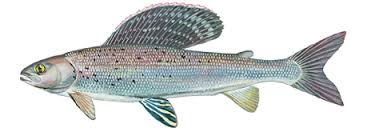
\includegraphics[keepaspectratio]{images/grayling.jpeg}}}{}}\label{section}

\section{What did we do last time?}\label{what-did-we-do-last-time}

\begin{itemize}
\item
  Implement data pipeline best practices
\item
  Apply controlled vocabulary and naming conventions
\item
  Create effective visualizations
\item
  Customize plots for publication quality
\item
  Combine multiple plots into composite figures

\begin{Shaded}
\begin{Highlighting}[]
\FunctionTok{ggplot}\NormalTok{(name\_df, }\FunctionTok{aes}\NormalTok{(x\_variable, y\_variable, }\AttributeTok{color =}\NormalTok{ categorical\_variable)) }\SpecialCharTok{+}
\CommentTok{\#      dataframe, aesthetics(x and y variables, mapping of color or fill or shape) + }
  \FunctionTok{geom\_point}\NormalTok{() }\SpecialCharTok{+}
\CommentTok{\# this it the geometry you want and can add more layers like}
  \FunctionTok{geom\_line}\NormalTok{()}
\end{Highlighting}
\end{Shaded}
\item
  What questions do you have and what is unclear
\item
  What did not work so far when you started the homework?
\end{itemize}

\section{Objectives and goals for
today}\label{objectives-and-goals-for-today}

\subsection{Today's Objectives}\label{todays-objectives}

\begin{enumerate}
\def\labelenumi{\arabic{enumi}.}
\tightlist
\item
  Implement descriptive statistics in R
\item
  Calculate measures of central tendency and spread
\item
  Compare distributions of data from different groups
\item
  Create effective visualizations of descriptive statistics
\item
  Interpret the meaning of these statistics in a biological context
\end{enumerate}

\pandocbounded{\includegraphics[keepaspectratio]{images/clipboard-2773654510.png}}

\section{Part 1: Setting Up Your
Environment}\label{part-1-setting-up-your-environment}

First, let's load the necessary packages and import our data:

\begin{Shaded}
\begin{Highlighting}[]
\CommentTok{\# Load required packages}

\FunctionTok{library}\NormalTok{(knitr)        }\CommentTok{\# For creating tables}
\FunctionTok{library}\NormalTok{(moments)      }\CommentTok{\# For calculating skewness and kurtosis}
\FunctionTok{library}\NormalTok{(skimr)        }\CommentTok{\# for summary stats}
\FunctionTok{library}\NormalTok{(flextable)    }\CommentTok{\# for tables if you want {-} now tinytable}
\FunctionTok{library}\NormalTok{(tidyverse)    }\CommentTok{\# For data wrangling and visualization}
\end{Highlighting}
\end{Shaded}

\begin{verbatim}
-- Attaching core tidyverse packages ------------------------ tidyverse 2.0.0 --
v dplyr     1.1.4     v readr     2.1.5
v forcats   1.0.0     v stringr   1.5.1
v ggplot2   3.5.2     v tibble    3.3.0
v lubridate 1.9.4     v tidyr     1.3.1
v purrr     1.1.0     
-- Conflicts ------------------------------------------ tidyverse_conflicts() --
x purrr::compose() masks flextable::compose()
x dplyr::filter()  masks stats::filter()
x dplyr::lag()     masks stats::lag()
i Use the conflicted package (<http://conflicted.r-lib.org/>) to force all conflicts to become errors
\end{verbatim}

\begin{Shaded}
\begin{Highlighting}[]
\CommentTok{\# Set a consistent theme for our plots}
\FunctionTok{theme\_set}\NormalTok{(}\FunctionTok{theme\_minimal}\NormalTok{(}\AttributeTok{base\_size =} \DecValTok{12}\NormalTok{))}
\end{Highlighting}
\end{Shaded}

\subsection{Getting the data}\label{getting-the-data}

\begin{tcolorbox}[enhanced jigsaw, opacitybacktitle=0.6, breakable, colbacktitle=quarto-callout-tip-color!10!white, toptitle=1mm, arc=.35mm, titlerule=0mm, title=\textcolor{quarto-callout-tip-color}{\faLightbulb}\hspace{0.5em}{Practice Exercise 1: Loading and Examining the Grayling Data}, coltitle=black, bottomrule=.15mm, rightrule=.15mm, colframe=quarto-callout-tip-color-frame, bottomtitle=1mm, toprule=.15mm, leftrule=.75mm, opacityback=0, left=2mm, colback=white]

We'll be working with data on arctic grayling fish from two different
lakes (I3 and I8).

\begin{Shaded}
\begin{Highlighting}[]
\CommentTok{\# Write your code here to read in the file}
\CommentTok{\# How do you examine the data {-} what are the ways you think and lets try it!}

\CommentTok{\# Load the grayling data}
\NormalTok{g\_df }\OtherTok{\textless{}{-}} \FunctionTok{read\_csv}\NormalTok{(}\StringTok{"data/gray\_I3\_I8.csv"}\NormalTok{)}
\end{Highlighting}
\end{Shaded}

\begin{verbatim}
Rows: 168 Columns: 5
-- Column specification --------------------------------------------------------
Delimiter: ","
chr (2): lake, species
dbl (3): site, length_mm, mass_g

i Use `spec()` to retrieve the full column specification for this data.
i Specify the column types or set `show_col_types = FALSE` to quiet this message.
\end{verbatim}

\begin{Shaded}
\begin{Highlighting}[]
\CommentTok{\# View the first few rows}
\FunctionTok{head}\NormalTok{(g\_df)}
\end{Highlighting}
\end{Shaded}

\begin{verbatim}
# A tibble: 6 x 5
   site lake  species         length_mm mass_g
  <dbl> <chr> <chr>               <dbl>  <dbl>
1   113 I3    arctic grayling       266    135
2   113 I3    arctic grayling       290    185
3   113 I3    arctic grayling       262    145
4   113 I3    arctic grayling       275    160
5   113 I3    arctic grayling       240    105
6   113 I3    arctic grayling       265    145
\end{verbatim}

\end{tcolorbox}

\begin{Shaded}
\begin{Highlighting}[]
\CommentTok{\# Examine the data structure}
\FunctionTok{glimpse}\NormalTok{(g\_df)}
\end{Highlighting}
\end{Shaded}

\begin{verbatim}
Rows: 168
Columns: 5
$ site      <dbl> 113, 113, 113, 113, 113, 113, 113, 113, 113, 113, 113, 113, ~
$ lake      <chr> "I3", "I3", "I3", "I3", "I3", "I3", "I3", "I3", "I3", "I3", ~
$ species   <chr> "arctic grayling", "arctic grayling", "arctic grayling", "ar~
$ length_mm <dbl> 266, 290, 262, 275, 240, 265, 265, 253, 246, 203, 289, 239, ~
$ mass_g    <dbl> 135, 185, 145, 160, 105, 145, 150, 130, 130, 71, 179, 108, 1~
\end{verbatim}

\begin{Shaded}
\begin{Highlighting}[]
\CommentTok{\# Get a statistical summary}
\FunctionTok{summary}\NormalTok{(g\_df)}
\end{Highlighting}
\end{Shaded}

\begin{verbatim}
      site         lake             species            length_mm    
 Min.   :113   Length:168         Length:168         Min.   :191.0  
 1st Qu.:113   Class :character   Class :character   1st Qu.:270.8  
 Median :118   Mode  :character   Mode  :character   Median :324.5  
 Mean   :116                                         Mean   :324.5  
 3rd Qu.:118                                         3rd Qu.:377.0  
 Max.   :118                                         Max.   :440.0  
                                                                    
     mass_g     
 Min.   : 53.0  
 1st Qu.:151.2  
 Median :340.0  
 Mean   :351.2  
 3rd Qu.:519.5  
 Max.   :889.0  
 NA's   :2      
\end{verbatim}

\begin{Shaded}
\begin{Highlighting}[]
\CommentTok{\# How many fish do we have from each lake?}

\NormalTok{g\_df }\SpecialCharTok{\%\textgreater{}\%}
  \FunctionTok{count}\NormalTok{(lake) }
\end{Highlighting}
\end{Shaded}

\begin{verbatim}
# A tibble: 2 x 2
  lake      n
  <chr> <int>
1 I3       66
2 I8      102
\end{verbatim}

\section{Questions to Consider:}\label{questions-to-consider}

\begin{enumerate}
\def\labelenumi{\arabic{enumi}.}
\tightlist
\item
  What variables are in our dataset?
\item
  What are their data types?
\item
  Are there any missing values?
\item
  What is the range of fish lengths in our dataset?
\item
  How many fish were sampled from each lake?
\end{enumerate}

\section{Part 2: Calculating Descriptive
Statistics}\label{part-2-calculating-descriptive-statistics}

\subsection{Let's calculate various descriptive statistics for our
data:}\label{lets-calculate-various-descriptive-statistics-for-our-data}

\subsection{}\label{section-1}

\begin{tcolorbox}[enhanced jigsaw, opacitybacktitle=0.6, breakable, colbacktitle=quarto-callout-tip-color!10!white, toptitle=1mm, arc=.35mm, titlerule=0mm, title=\textcolor{quarto-callout-tip-color}{\faLightbulb}\hspace{0.5em}{Practice Exercise 2: Measures of Central Tendency}, coltitle=black, bottomrule=.15mm, rightrule=.15mm, colframe=quarto-callout-tip-color-frame, bottomtitle=1mm, toprule=.15mm, leftrule=.75mm, opacityback=0, left=2mm, colback=white]

Let's recreate the basic histogram of fish lengths from our last class.
Use the \texttt{sculpin\_df} data frame that's already loaded.

\begin{Shaded}
\begin{Highlighting}[]
\CommentTok{\# Write your code here to read in the file}
\CommentTok{\# How do you examine the data {-} what are the ways you think and lets try it!}
\CommentTok{\# Calculate the mean and median fish length}
\FunctionTok{mean}\NormalTok{(g\_df}\SpecialCharTok{$}\NormalTok{length\_mm)}
\end{Highlighting}
\end{Shaded}

\begin{verbatim}
[1] 324.494
\end{verbatim}

\begin{Shaded}
\begin{Highlighting}[]
\FunctionTok{median}\NormalTok{(g\_df}\SpecialCharTok{$}\NormalTok{length\_mm)}
\end{Highlighting}
\end{Shaded}

\begin{verbatim}
[1] 324.5
\end{verbatim}

\end{tcolorbox}

\begin{Shaded}
\begin{Highlighting}[]
\CommentTok{\# Calculate mean and median by lake}
\NormalTok{g\_df }\SpecialCharTok{\%\textgreater{}\%}
  \FunctionTok{group\_by}\NormalTok{(lake) }\SpecialCharTok{\%\textgreater{}\%}
  \FunctionTok{summarise}\NormalTok{(}
    \AttributeTok{mean\_length =} \FunctionTok{mean}\NormalTok{(length\_mm),}
    \AttributeTok{median\_length =} \FunctionTok{median}\NormalTok{(length\_mm)}
\NormalTok{  ) }
\end{Highlighting}
\end{Shaded}

\begin{verbatim}
# A tibble: 2 x 3
  lake  mean_length median_length
  <chr>       <dbl>         <dbl>
1 I3           266.           266
2 I8           363.           373
\end{verbatim}

\subsection{Summarizing data - two
ways}\label{summarizing-data---two-ways}

lets say we want to summarize the data and need to get n, means,
standard deviation, standard error

We could do the following - if we had missing cells the code below would
give an error

\begin{Shaded}
\begin{Highlighting}[]
\FunctionTok{mean}\NormalTok{(g\_df}\SpecialCharTok{$}\NormalTok{length\_mm) }
\end{Highlighting}
\end{Shaded}

\begin{verbatim}
[1] 324.494
\end{verbatim}

\begin{Shaded}
\begin{Highlighting}[]
\FunctionTok{mean}\NormalTok{(g\_df}\SpecialCharTok{$}\NormalTok{length\_mm, }\AttributeTok{na.rm =} \ConstantTok{TRUE}\NormalTok{) }\CommentTok{\# removes missing values}
\end{Highlighting}
\end{Shaded}

\begin{verbatim}
[1] 324.494
\end{verbatim}

\begin{Shaded}
\begin{Highlighting}[]
\FunctionTok{length}\NormalTok{(g\_df}\SpecialCharTok{$}\NormalTok{length\_mm)}
\end{Highlighting}
\end{Shaded}

\begin{verbatim}
[1] 168
\end{verbatim}

\begin{itemize}
\item
  \textbf{the length counts missing and non-missing data}
\item
  however this would get old if we had to do this for everything and
  then to do it for the different groupings - lee and windward\ldots{}
\end{itemize}

\subsection{We need to learn to pipe}\label{we-need-to-learn-to-pipe}

\subsubsection{passes things from the dataframe to a command and so
on\ldots{}}\label{passes-things-from-the-dataframe-to-a-command-and-so-on}

\begin{itemize}
\tightlist
\item
  the dataframe --\textgreater{} pipe command that feed the dataframe
  into --\textgreater{} next command
\end{itemize}

\begin{Shaded}
\begin{Highlighting}[]
\NormalTok{g\_df }\SpecialCharTok{\%\textgreater{}\%} \FunctionTok{summarize}\NormalTok{(}\AttributeTok{mean\_length =} \FunctionTok{mean}\NormalTok{(length\_mm, }\AttributeTok{na.rm =} \ConstantTok{TRUE}\NormalTok{))}
\end{Highlighting}
\end{Shaded}

\begin{verbatim}
# A tibble: 1 x 1
  mean_length
        <dbl>
1        324.
\end{verbatim}

\subsection{What is cool is we can do a lot of different things
now}\label{what-is-cool-is-we-can-do-a-lot-of-different-things-now}

\begin{Shaded}
\begin{Highlighting}[]
\NormalTok{g\_df }\SpecialCharTok{\%\textgreater{}\%} 
  \FunctionTok{summarize}\NormalTok{(}
    \AttributeTok{mean\_length =} \FunctionTok{mean}\NormalTok{(length\_mm, }\AttributeTok{na.rm =} \ConstantTok{TRUE}\NormalTok{),}
    \AttributeTok{sd\_length =} \FunctionTok{sd}\NormalTok{(length\_mm, }\AttributeTok{na.rm =} \ConstantTok{TRUE}\NormalTok{),}
    \AttributeTok{n\_length =} \FunctionTok{n}\NormalTok{())}
\end{Highlighting}
\end{Shaded}

\begin{verbatim}
# A tibble: 1 x 3
  mean_length sd_length n_length
        <dbl>     <dbl>    <int>
1        324.      65.0      168
\end{verbatim}

\subsection{Super cool code in case there are missing
values}\label{super-cool-code-in-case-there-are-missing-values}

\begin{Shaded}
\begin{Highlighting}[]
\NormalTok{g\_df }\SpecialCharTok{\%\textgreater{}\%} 
  \FunctionTok{summarize}\NormalTok{(}
    \AttributeTok{mean\_length =} \FunctionTok{mean}\NormalTok{(length\_mm, }\AttributeTok{na.rm =} \ConstantTok{TRUE}\NormalTok{),}
    \AttributeTok{sd\_length =} \FunctionTok{sd}\NormalTok{(length\_mm, }\AttributeTok{na.rm =} \ConstantTok{TRUE}\NormalTok{),}
    \AttributeTok{n\_length =} \FunctionTok{sum}\NormalTok{(}\SpecialCharTok{!}\FunctionTok{is.na}\NormalTok{(length\_mm)))}
\end{Highlighting}
\end{Shaded}

\begin{verbatim}
# A tibble: 1 x 3
  mean_length sd_length n_length
        <dbl>     <dbl>    <int>
1        324.      65.0      168
\end{verbatim}

\section{Now for Spread\ldots{}}\label{now-for-spread}

\begin{tcolorbox}[enhanced jigsaw, opacitybacktitle=0.6, breakable, colbacktitle=quarto-callout-tip-color!10!white, toptitle=1mm, arc=.35mm, titlerule=0mm, title=\textcolor{quarto-callout-tip-color}{\faLightbulb}\hspace{0.5em}{Practice Exercise 3: Measures of Spread}, coltitle=black, bottomrule=.15mm, rightrule=.15mm, colframe=quarto-callout-tip-color-frame, bottomtitle=1mm, toprule=.15mm, leftrule=.75mm, opacityback=0, left=2mm, colback=white]

\begin{Shaded}
\begin{Highlighting}[]
\CommentTok{\# Write your code here to read in the file}
\CommentTok{\# Calculate standard deviation and variance}
\NormalTok{mean\_length }\OtherTok{\textless{}{-}} \FunctionTok{mean}\NormalTok{(g\_df}\SpecialCharTok{$}\NormalTok{length\_mm, }\AttributeTok{na.rm=}\ConstantTok{TRUE}\NormalTok{)}
\NormalTok{sd\_length }\OtherTok{\textless{}{-}} \FunctionTok{sd}\NormalTok{(g\_df}\SpecialCharTok{$}\NormalTok{length\_mm)}
\NormalTok{var\_length }\OtherTok{\textless{}{-}} \FunctionTok{var}\NormalTok{(g\_df}\SpecialCharTok{$}\NormalTok{length\_mm)}
\NormalTok{sd\_length}
\end{Highlighting}
\end{Shaded}

\begin{verbatim}
[1] 65.00659
\end{verbatim}

\begin{Shaded}
\begin{Highlighting}[]
\NormalTok{var\_length}
\end{Highlighting}
\end{Shaded}

\begin{verbatim}
[1] 4225.856
\end{verbatim}

\end{tcolorbox}

\begin{tcolorbox}[enhanced jigsaw, opacitybacktitle=0.6, breakable, colbacktitle=quarto-callout-tip-color!10!white, toptitle=1mm, arc=.35mm, titlerule=0mm, title=\textcolor{quarto-callout-tip-color}{\faLightbulb}\hspace{0.5em}{Exercise 4: Calculate Quartiles and Percentiles}, coltitle=black, bottomrule=.15mm, rightrule=.15mm, colframe=quarto-callout-tip-color-frame, bottomtitle=1mm, toprule=.15mm, leftrule=.75mm, opacityback=0, left=2mm, colback=white]

\begin{Shaded}
\begin{Highlighting}[]
\CommentTok{\# Calculate quartiles for overall data}
\NormalTok{quartiles }\OtherTok{\textless{}{-}} \FunctionTok{quantile}\NormalTok{(g\_df}\SpecialCharTok{$}\NormalTok{length\_mm, }\AttributeTok{probs =} \FunctionTok{c}\NormalTok{(}\FloatTok{0.25}\NormalTok{, }\FloatTok{0.5}\NormalTok{, }\FloatTok{0.75}\NormalTok{))}
\CommentTok{\# cat("First quartile (Q1):", quartiles[1], "mm\textbackslash{}n")}
\CommentTok{\# cat("Second quartile (Median):", quartiles[2], "mm\textbackslash{}n")}
\CommentTok{\# cat("Third quartile (Q3):", quartiles[3], "mm\textbackslash{}n")}

\CommentTok{\# Calculate a more comprehensive set of percentiles}
\NormalTok{percentiles }\OtherTok{\textless{}{-}} \FunctionTok{quantile}\NormalTok{(g\_df}\SpecialCharTok{$}\NormalTok{length\_mm, }
                        \AttributeTok{probs =} \FunctionTok{c}\NormalTok{(}\FloatTok{0.1}\NormalTok{, }\FloatTok{0.25}\NormalTok{, }\FloatTok{0.5}\NormalTok{, }\FloatTok{0.75}\NormalTok{, }\FloatTok{0.9}\NormalTok{))}

\CommentTok{\# Display the percentiles using flextable}
\FunctionTok{data.frame}\NormalTok{(}
  \AttributeTok{Percentile =} \FunctionTok{c}\NormalTok{(}\StringTok{"10th"}\NormalTok{, }\StringTok{"25th (Q1)"}\NormalTok{, }\StringTok{"50th (Median)"}\NormalTok{, }\StringTok{"75th (Q3)"}\NormalTok{, }\StringTok{"90th"}\NormalTok{),}
  \AttributeTok{Value =}\NormalTok{ percentiles}
\NormalTok{) }
\end{Highlighting}
\end{Shaded}

\begin{verbatim}
       Percentile  Value
10%          10th 251.10
25%     25th (Q1) 270.75
50% 50th (Median) 324.50
75%     75th (Q3) 377.00
90%          90th 408.60
\end{verbatim}

\end{tcolorbox}

\subsubsection{Note you could add a box plot by lake to see this if you
wanted}\label{note-you-could-add-a-box-plot-by-lake-to-see-this-if-you-wanted}

\begin{Shaded}
\begin{Highlighting}[]
\NormalTok{g\_df }\SpecialCharTok{\%\textgreater{}\%} 
  \FunctionTok{ggplot}\NormalTok{(}\FunctionTok{aes}\NormalTok{(lake, length\_mm, }\AttributeTok{color=}\NormalTok{ lake))}\SpecialCharTok{+}
  \FunctionTok{geom\_boxplot}\NormalTok{()}
\end{Highlighting}
\end{Shaded}

\pandocbounded{
\includegraphics[keepaspectratio]{03_02_class_activity_files/figure-pdf/boxplot-1.pdf}}

\begin{tcolorbox}[enhanced jigsaw, opacitybacktitle=0.6, breakable, colbacktitle=quarto-callout-tip-color!10!white, toptitle=1mm, arc=.35mm, titlerule=0mm, title=\textcolor{quarto-callout-tip-color}{\faLightbulb}\hspace{0.5em}{Exercise 5: Calculate the Coefficient of Variation}, coltitle=black, bottomrule=.15mm, rightrule=.15mm, colframe=quarto-callout-tip-color-frame, bottomtitle=1mm, toprule=.15mm, leftrule=.75mm, opacityback=0, left=2mm, colback=white]

The coefficient of variation (CV) is the standard deviation expressed as
a percentage of the mean:

\[CV = \frac{s}{\bar{Y}} \times 100\%\]

\begin{Shaded}
\begin{Highlighting}[]
\CommentTok{\# Calculate coefficient of variation}
\NormalTok{sd\_length }\SpecialCharTok{/}\NormalTok{ mean\_length }\SpecialCharTok{*} \DecValTok{100}
\end{Highlighting}
\end{Shaded}

\begin{verbatim}
[1] 20.03321
\end{verbatim}

\end{tcolorbox}

\begin{Shaded}
\begin{Highlighting}[]
\CommentTok{\# Calculate by lake}
\NormalTok{g\_df }\SpecialCharTok{\%\textgreater{}\%}
  \FunctionTok{group\_by}\NormalTok{(lake) }\SpecialCharTok{\%\textgreater{}\%}
  \FunctionTok{summarise}\NormalTok{(}
    \AttributeTok{mean\_length =} \FunctionTok{mean}\NormalTok{(length\_mm),}
    \AttributeTok{sd\_length =} \FunctionTok{sd}\NormalTok{(length\_mm),}
    \AttributeTok{cv\_length =}\NormalTok{ sd\_length }\SpecialCharTok{/}\NormalTok{ mean\_length }\SpecialCharTok{*} \DecValTok{100}
\NormalTok{  ) }\SpecialCharTok{\%\textgreater{}\%}
  \FunctionTok{flextable}\NormalTok{()}
\end{Highlighting}
\end{Shaded}

\global\setlength{\Oldarrayrulewidth}{\arrayrulewidth}

\global\setlength{\Oldtabcolsep}{\tabcolsep}

\setlength{\tabcolsep}{2pt}

\renewcommand*{\arraystretch}{1.5}



\providecommand{\ascline}[3]{\noalign{\global\arrayrulewidth #1}\arrayrulecolor[HTML]{#2}\cline{#3}}

\begin{longtable*}[c]{|p{0.75in}|p{0.75in}|p{0.75in}|p{0.75in}}



\ascline{1.5pt}{666666}{1-4}

\multicolumn{1}{>{\raggedright}m{\dimexpr 0.75in+0\tabcolsep}}{\textcolor[HTML]{000000}{\fontsize{11}{11}\selectfont{\global\setmainfont{Helvetica}{lake}}}} & \multicolumn{1}{>{\raggedleft}m{\dimexpr 0.75in+0\tabcolsep}}{\textcolor[HTML]{000000}{\fontsize{11}{11}\selectfont{\global\setmainfont{Helvetica}{mean\_length}}}} & \multicolumn{1}{>{\raggedleft}m{\dimexpr 0.75in+0\tabcolsep}}{\textcolor[HTML]{000000}{\fontsize{11}{11}\selectfont{\global\setmainfont{Helvetica}{sd\_length}}}} & \multicolumn{1}{>{\raggedleft}m{\dimexpr 0.75in+0\tabcolsep}}{\textcolor[HTML]{000000}{\fontsize{11}{11}\selectfont{\global\setmainfont{Helvetica}{cv\_length}}}} \\

\ascline{1.5pt}{666666}{1-4}\endfirsthead 

\ascline{1.5pt}{666666}{1-4}

\multicolumn{1}{>{\raggedright}m{\dimexpr 0.75in+0\tabcolsep}}{\textcolor[HTML]{000000}{\fontsize{11}{11}\selectfont{\global\setmainfont{Helvetica}{lake}}}} & \multicolumn{1}{>{\raggedleft}m{\dimexpr 0.75in+0\tabcolsep}}{\textcolor[HTML]{000000}{\fontsize{11}{11}\selectfont{\global\setmainfont{Helvetica}{mean\_length}}}} & \multicolumn{1}{>{\raggedleft}m{\dimexpr 0.75in+0\tabcolsep}}{\textcolor[HTML]{000000}{\fontsize{11}{11}\selectfont{\global\setmainfont{Helvetica}{sd\_length}}}} & \multicolumn{1}{>{\raggedleft}m{\dimexpr 0.75in+0\tabcolsep}}{\textcolor[HTML]{000000}{\fontsize{11}{11}\selectfont{\global\setmainfont{Helvetica}{cv\_length}}}} \\

\ascline{1.5pt}{666666}{1-4}\endhead



\multicolumn{1}{>{\raggedright}m{\dimexpr 0.75in+0\tabcolsep}}{\textcolor[HTML]{000000}{\fontsize{11}{11}\selectfont{\global\setmainfont{Helvetica}{I3}}}} & \multicolumn{1}{>{\raggedleft}m{\dimexpr 0.75in+0\tabcolsep}}{\textcolor[HTML]{000000}{\fontsize{11}{11}\selectfont{\global\setmainfont{Helvetica}{265.6061}}}} & \multicolumn{1}{>{\raggedleft}m{\dimexpr 0.75in+0\tabcolsep}}{\textcolor[HTML]{000000}{\fontsize{11}{11}\selectfont{\global\setmainfont{Helvetica}{28.30378}}}} & \multicolumn{1}{>{\raggedleft}m{\dimexpr 0.75in+0\tabcolsep}}{\textcolor[HTML]{000000}{\fontsize{11}{11}\selectfont{\global\setmainfont{Helvetica}{10.65630}}}} \\





\multicolumn{1}{>{\raggedright}m{\dimexpr 0.75in+0\tabcolsep}}{\textcolor[HTML]{000000}{\fontsize{11}{11}\selectfont{\global\setmainfont{Helvetica}{I8}}}} & \multicolumn{1}{>{\raggedleft}m{\dimexpr 0.75in+0\tabcolsep}}{\textcolor[HTML]{000000}{\fontsize{11}{11}\selectfont{\global\setmainfont{Helvetica}{362.5980}}}} & \multicolumn{1}{>{\raggedleft}m{\dimexpr 0.75in+0\tabcolsep}}{\textcolor[HTML]{000000}{\fontsize{11}{11}\selectfont{\global\setmainfont{Helvetica}{52.33901}}}} & \multicolumn{1}{>{\raggedleft}m{\dimexpr 0.75in+0\tabcolsep}}{\textcolor[HTML]{000000}{\fontsize{11}{11}\selectfont{\global\setmainfont{Helvetica}{14.43444}}}} \\

\ascline{1.5pt}{666666}{1-4}



\end{longtable*}



\arrayrulecolor[HTML]{000000}

\global\setlength{\arrayrulewidth}{\Oldarrayrulewidth}

\global\setlength{\tabcolsep}{\Oldtabcolsep}

\renewcommand*{\arraystretch}{1}

\subsubsection{Questions to Consider:}\label{questions-to-consider-1}

\begin{enumerate}
\def\labelenumi{\arabic{enumi}.}
\tightlist
\item
  How do the means and medians compare within each lake? What might this
  tell you about the distribution?
\item
  Which lake has more variable fish lengths? How can you tell?
\item
  Why might the coefficient of variation be useful when comparing
  variability between different measurements (e.g., length vs.~mass)?
\end{enumerate}

\subsection{Part 3: Visualizing
Distributions}\label{part-3-visualizing-distributions}

Visualizations can help us better understand the descriptive statistics
we've calculated.

\begin{tcolorbox}[enhanced jigsaw, opacitybacktitle=0.6, breakable, colbacktitle=quarto-callout-tip-color!10!white, toptitle=1mm, arc=.35mm, titlerule=0mm, title=\textcolor{quarto-callout-tip-color}{\faLightbulb}\hspace{0.5em}{Exercise 6: Creating Histograms}, coltitle=black, bottomrule=.15mm, rightrule=.15mm, colframe=quarto-callout-tip-color-frame, bottomtitle=1mm, toprule=.15mm, leftrule=.75mm, opacityback=0, left=2mm, colback=white]

One of the best ways to look at data is a histogram - and we will do it
again

\begin{Shaded}
\begin{Highlighting}[]
\CommentTok{\# Create a histogram of all fish lengths}
\NormalTok{g\_df }\SpecialCharTok{\%\textgreater{}\%} \FunctionTok{ggplot}\NormalTok{(}\FunctionTok{aes}\NormalTok{(}\AttributeTok{x =}\NormalTok{ length\_mm)) }\SpecialCharTok{+}
  \FunctionTok{geom\_histogram}\NormalTok{(}\AttributeTok{bins =} \DecValTok{15}\NormalTok{) }
\end{Highlighting}
\end{Shaded}

\pandocbounded{
\includegraphics[keepaspectratio]{03_02_class_activity_files/figure-pdf/histograms-1.pdf}}

\end{tcolorbox}

\subsubsection{}\label{section-2}

\begin{Shaded}
\begin{Highlighting}[]
\CommentTok{\# Create histograms by lake}
\NormalTok{g\_df  }\SpecialCharTok{\%\textgreater{}\%} \FunctionTok{ggplot}\NormalTok{(}\FunctionTok{aes}\NormalTok{(}\AttributeTok{x =}\NormalTok{ length\_mm, }\AttributeTok{fill =}\NormalTok{ lake)) }\SpecialCharTok{+}
  \FunctionTok{geom\_histogram}\NormalTok{(}\AttributeTok{bins =} \DecValTok{15}\NormalTok{, }\AttributeTok{position =} \StringTok{"dodge"}\NormalTok{, }\AttributeTok{alpha =} \FloatTok{0.7}\NormalTok{) }
\end{Highlighting}
\end{Shaded}

\pandocbounded{
\includegraphics[keepaspectratio]{03_02_class_activity_files/figure-pdf/unnamed-chunk-12-1.pdf}}

\begin{tcolorbox}[enhanced jigsaw, opacitybacktitle=0.6, breakable, colbacktitle=quarto-callout-tip-color!10!white, toptitle=1mm, arc=.35mm, titlerule=0mm, title=\textcolor{quarto-callout-tip-color}{\faLightbulb}\hspace{0.5em}{Exercise 7: Creating Box Plots}, coltitle=black, bottomrule=.15mm, rightrule=.15mm, colframe=quarto-callout-tip-color-frame, bottomtitle=1mm, toprule=.15mm, leftrule=.75mm, opacityback=0, left=2mm, colback=white]

Personally I like box plots

\begin{Shaded}
\begin{Highlighting}[]
\CommentTok{\# Create a box plot comparing fish lengths by lake}
\CommentTok{\# Create a box plot comparing fish lengths by lake}
\NormalTok{g\_df  }\SpecialCharTok{\%\textgreater{}\%}  \FunctionTok{ggplot}\NormalTok{( }\FunctionTok{aes}\NormalTok{(}\AttributeTok{x =}\NormalTok{ lake, }\AttributeTok{y =}\NormalTok{ length\_mm, }\AttributeTok{fill =}\NormalTok{ lake)) }\SpecialCharTok{+}
  \FunctionTok{geom\_boxplot}\NormalTok{() }
\end{Highlighting}
\end{Shaded}

\pandocbounded{
\includegraphics[keepaspectratio]{03_02_class_activity_files/figure-pdf/boxplots-1.pdf}}

\end{tcolorbox}

\subsubsection{}\label{section-3}

\begin{tcolorbox}[enhanced jigsaw, opacitybacktitle=0.6, breakable, colbacktitle=quarto-callout-tip-color!10!white, toptitle=1mm, arc=.35mm, titlerule=0mm, title=\textcolor{quarto-callout-tip-color}{\faLightbulb}\hspace{0.5em}{Exercise 9: Creating Density Plots}, coltitle=black, bottomrule=.15mm, rightrule=.15mm, colframe=quarto-callout-tip-color-frame, bottomtitle=1mm, toprule=.15mm, leftrule=.75mm, opacityback=0, left=2mm, colback=white]

Now these will be really important later on

\begin{Shaded}
\begin{Highlighting}[]
\DocumentationTok{\#\# Create density plots}
\NormalTok{g\_df  }\SpecialCharTok{\%\textgreater{}\%}  \FunctionTok{ggplot}\NormalTok{(}\FunctionTok{aes}\NormalTok{(}\AttributeTok{x =}\NormalTok{ length\_mm, }\AttributeTok{fill =}\NormalTok{ lake)) }\SpecialCharTok{+}
  \FunctionTok{geom\_density}\NormalTok{(}\AttributeTok{alpha =} \FloatTok{0.5}\NormalTok{)}
\end{Highlighting}
\end{Shaded}

\pandocbounded{
\includegraphics[keepaspectratio]{03_02_class_activity_files/figure-pdf/density-plots-1.pdf}}

\end{tcolorbox}

\subsubsection{}\label{section-4}

\subsubsection{Questions to Consider:}\label{questions-to-consider-2}

\begin{enumerate}
\def\labelenumi{\arabic{enumi}.}
\tightlist
\item
  Which visualization best shows the differences in fish lengths between
  lakes?
\item
  What can you learn from the violin plots that might not be apparent
  from the box plots?
\item
  How would you interpret the cumulative frequency distribution?
\item
  What patterns or insights can you identify from these visualizations?
\end{enumerate}

\subsection{Part 4: Interpreting the
Results}\label{part-4-interpreting-the-results}

Based on our analysis, we can make the following observations:

\begin{enumerate}
\def\labelenumi{\arabic{enumi}.}
\item
  \textbf{Lake Differences}: Fish from Lake I8 are generally larger than
  those from Lake I3, both in length and mass.
\item
  \textbf{Variability}: Lake I8 shows greater variability in fish
  lengths and masses than Lake I3, as indicated by higher standard
  deviations and IQRs.
\item
  \textbf{Distribution Shape}:

  \begin{itemize}
  \tightlist
  \item
    Lake I3 fish lengths are more symmetrically distributed.
  \item
    Lake I8 fish lengths show a slight negative skew, suggesting a few
    smaller fish pulling the distribution to the left.
  \end{itemize}
\item
  \textbf{Length-Mass Relationship}: Both lakes show a strong positive
  correlation between fish length and mass, following an approximately
  cubic relationship (mass increases with the cube of length).
\end{enumerate}

\subsection{Guided Questions for Deeper Understanding of descriptive
statistics}\label{guided-questions-for-deeper-understanding-of-descriptive-statistics}

\begin{enumerate}
\def\labelenumi{\arabic{enumi}.}
\item
  \textbf{Biological Interpretation}: What ecological factors might
  explain the differences in fish size between the two lakes?
\item
  \textbf{Statistical Reasoning}: Why might we prefer to use the median
  and IQR instead of the mean and standard deviation in some cases?
\item
  \textbf{Data Visualization}: Which visualization method was most
  effective for comparing the two lakes? Why?
\item
  \textbf{Scientific Communication}: How would you concisely summarize
  these findings in a scientific paper?
\item
  \textbf{Further Analysis}: What additional analyses might be useful to
  better understand this dataset?
\end{enumerate}




\end{document}
